\documentclass[10pt]{amsart}

\usepackage{graphicx}
\usepackage{minted}

% \usemintedstyle{rainbow_dash}

\author{Arden Rasmussen}
\title{Computational Physics Final}
\date{\today}

\begin{document}
\maketitle
\section{Lorenz Attractor}%
\label{sec:lorenz_attractor}

\centering
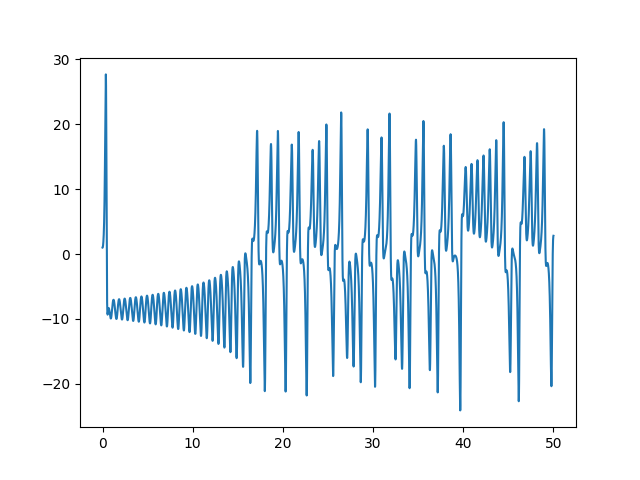
\includegraphics[width=0.8\linewidth]{../P1_a.png}

\centering
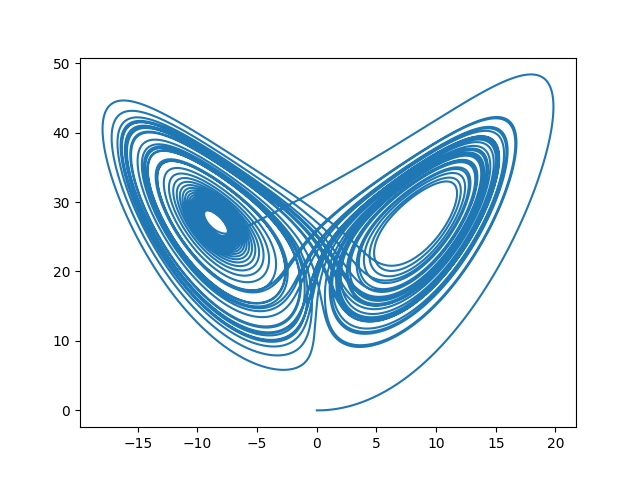
\includegraphics[width=0.8\linewidth]{../P1_b.png}

\section{The Electric Potential of a Square Wire}%
\label{sec:the_electric_potential_of_a_square_wire}

\begin{align*}
    V(0,0) &= 7.050987223017098\\
    V\left(\frac{1}{4},0\right) &= 7.489509173680615
\end{align*}

\begin{align*}
    \vec{E}(0,0) &= \begin{pmatrix}
       0.0 \\ 0.0
    \end{pmatrix}\\
    \vec{E}\left(\frac{1}{4},0\right) &= \begin{pmatrix}
      4.3173101895277455 \\  4.4408920985006255\cdot10^{-11}
    \end{pmatrix}
\end{align*}

\centering
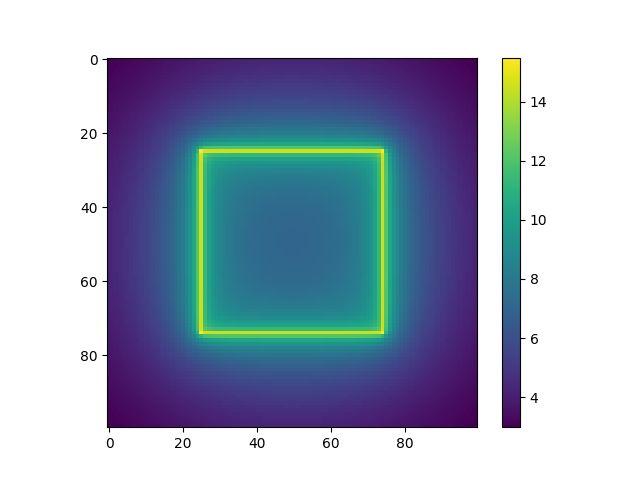
\includegraphics[width=0.8\linewidth]{../P2_4.png}

\section{The Potential in the Presence of Boundaries}%
\label{sec:the_potential_in_the_presence_of_boundaries}

\begin{align*}
    V(0,0) &= 0.012354418658953788\\
    V\left(\frac{1}{4},0\right) &= 0.016312469694817238
\end{align*}

\begin{align*}
    \vec{E}(0,0) &= \begin{pmatrix}
       0.011806814924191639 \\ 0.011806814924191465
    \end{pmatrix}\\
    \vec{E}\left(\frac{1}{4},0\right) &= \begin{pmatrix}
      0.011079095703054806 \\  0.009159891802292333
    \end{pmatrix}
\end{align*}

\centering
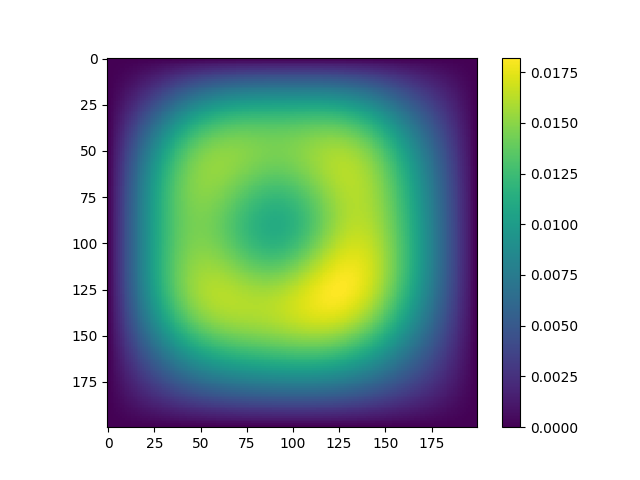
\includegraphics[width=0.8\linewidth]{../P3_3.png}


\appendix
\newpage
\section{Lorenz Attractor}%
\label{sec:lorenz_attractor}

\inputminted[linenos]{python}{../P1.py}

\newpage
\section{The Electric Potential of a Square Wire}%
\label{sec:the_electric_potential_of_a_square_wire}

\inputminted[linenos]{python}{../P2.py}

\newpage
\section{The Potential in the Presence of Boundaries}%
\label{sec:the_potential_in_the_presence_of_boundaries}

\inputminted[linenos]{python}{../P3.py}

\end{document}
